\documentclass[11pt]{article}

\usepackage[letterpaper, margin=1in]{geometry}

\usepackage[utf8]{inputenc}
\usepackage[spanish]{babel}
\usepackage{multirow}
\usepackage{tabularx}
\usepackage{longtable}

%Figuras
\usepackage{graphicx, subfigure}
\usepackage[]{tikz}
\usepackage{pbox}

%Matemática
\usepackage{amsmath}
\usepackage{amssymb}

%Símbolos mate extra (alfabetos, etc.)
\usepackage{mathrsfs}


%Algoritmos
\usepackage{float}
\usepackage{algorithm}
\usepackage{algorithmicx}
\usepackage{algpseudocode}
\usepackage{listings} %Para Código
\usepackage{listingsutf8}


\usepackage{color}
\usepackage{hyperref}

\usepackage{mdframed}
\usepackage{tcolorbox}
\usepackage{multicol}
\usepackage{booktabs}
\usepackage{tabulary}
\definecolor{darkblue}{rgb}{0 , 0.054 , 0.196}


\title{Reporte de Laboratorio 2\\Herencia, polimorfísmo y sobrecargas en C++}
\author{Dunia Barahona - B40806}
%otro autor se pondría así \author{nombre1\\nombre2}
\begin{document}

\maketitle
\hrule
\hrule
\tableofcontents
\hspace{5mm}
\hrule
\hrule

\section{Código}
\lstset{inputencoding=utf8/latin1}

\subsection{Clase Base: Figura}
\subsubsection*{Figura.h}
\begin{lstlisting}
#ifndef FIGURA_H
#define FIGURA_H

#include <cstdlib>
#include <iostream>
#include "math.h"
#include "string"

using namespace std;

class Figura{ //Clase base
public:
	string color; // atributos...
	string nombre;
	
	Figura();	
	Figura(string nombre, string color);
	virtual ~Figura(); //destructor...
	
	virtual double area(); //virtuales...
	virtual double pmt();
	
	virtual void operator~(); //sobrecarga de operadores...
	virtual void operator!();
};
#endif /* FIGURA_H */
\end{lstlisting}
\vspace{1 em}
\subsubsection*{Figura.cpp}
\begin{lstlisting}
#include "Figura.h"

Figura::Figura() {  //constructores
}
Figura::Figura(string nombre, string color) {
	this->nombre = nombre;
	this->color = color;
}
Figura::~Figura() {  //destructor
}

//virtuales: que se reimplementaran en las clases derivadas
double Figura::area() {  
	cout << "Metodo para calcular el area de la figura"<<
	this->nombre<< "debe implementarse en clases derivadas." << endl;
	return 0.0;
}
double Figura::pmt() { 
	cout << "Metodo para calcular el perimetro de la figura"<<
	this->nombre<< "debe implementarse en clases derivadas." << endl;
	return 0.0;
}
void Figura::operator ~() {  //imprime los atributos del objeto.
	cout << "Nombre: "<< this->nombre << endl;
	cout << "Color:  " <<this->color << endl;
}
void Figura::operator !() {  //imprime el area y perimetro de la figura
	cout << "Area:   "<< this->area() << endl;
	cout << "Perímetro: "<< this->pmt() << endl;
	cout << endl;
}
\end{lstlisting}
\newpage
\subsection{Clase derivada: Círculo}
\subsubsection*{Circulo.h}
\begin{lstlisting}.
#ifndef CIRCULO_H
#define CIRCULO_H

#include "Figura.h"

//Clase 'Circulo' que hereda publicamente de la clase 'Figura'
class Circulo : public Figura{
public:
	double radio; //atributo propio...
	Circulo();
	Circulo(string nombre, string color, double radio);
	virtual ~Circulo(); //destructor...
	
	virtual double area(); 	//reimplementados...
	virtual double pmt();
	
	virtual void operator~(); //sobrecarga de operadores...
	virtual void operator!();
};
#endif /* CIRCULO_H */	
\end{lstlisting}
\vspace{1 em}
\subsubsection*{Circulo.cpp}
\begin{lstlisting}
#include "Circulo.h"

Circulo::Circulo() {		
}
Circulo::Circulo(string nombre, string color, double radio) {
	this->nombre =nombre;
	this->color =color;
	this->radio =radio;
}
Circulo::~Circulo() {
}
double Circulo::area() {
	double r= this->radio;
	double a= 3.1415*(r*r);
	return a;
}
double Circulo::pmt() {
	double r= this->radio;
	double p= 2*3.1415*r;
	return p;
}
void Circulo::operator ~() {
	cout << "Nombre: "<<this->nombre << endl;
	cout << "Color:  " <<this->color << endl;
	cout << "Radio:  "<<this->radio << " cm"<<endl;
}
void Circulo::operator !() { 
	cout << "Area:   "<<this->area()<<endl;
	cout << "Perimetro: "<<this->pmt() <<endl;
	cout << endl;
}
\end{lstlisting}
\vspace{2 em}

\subsection{Clase derivada: Cuadrado}
\subsubsection*{Cuadrado.h}
\begin{lstlisting}
#ifndef CUADRADO_H
#define CUADRADO_H

#include "Figura.h"

//Clase 'Cuadrado' que hereda publicamente de la clase 'Figura'
class Cuadrado : public Figura {	
public:
	double lado; //atributo propio...
	Cuadrado();
	Cuadrado(string nombre, string color, double lado);
	virtual ~Cuadrado(); //destructor...
	
	virtual double area(); //reimplementados...
	virtual double pmt();
	
	virtual void operator~(); //sobrecarga de operadores...
	virtual void operator!();
};
#endif /* CUADRADO_H */
\end{lstlisting}
\vspace{1 em}
\subsubsection*{Cuadrado.cpp}
\begin{lstlisting}
#include "Cuadrado.h"

Cuadrado::Cuadrado() {	
}
Cuadrado::Cuadrado(string nombre, string color, double lado) {
	this->nombre =nombre;
	this->color =color;
	this->lado =lado;		
}
Cuadrado::~Cuadrado() { //destructor
}
double Cuadrado::area() {
	double l= this->lado;
	double a= l*l;
	return a;
}
double Cuadrado::pmt() {
	double l= this->lado;
	double p= 4*l;
	return p;
}
void Cuadrado::operator ~() {
	cout << "Nombre: "<<this->nombre << endl;
	cout << "Color:  "<<this->color << endl;
	cout << "Longitud de lado: "<<this->lado << " cm"<<endl;
}
void Cuadrado::operator !() { 
	cout << "Area:   "<<this->area() << endl;
	cout << "Perimetro: "<<this->pmt() << endl;
	cout << endl;
}

\end{lstlisting}
\vspace{2 em}

\subsection{Clase derivada: Triángulo}
\subsubsection*{Triangulo.h}
\begin{lstlisting}
#ifndef TRIANGULO_H
#define TRIANGULO_H
	
#include "Figura.h"
	
// Clase 'Triangulo' que hereda publicamente de la clase 'Figura'
class Triangulo : public Figura{	
public:
	double lado_1; //atributos propios: lados del triangulo...
	double lado_2;
	double lado_3;
	Triangulo();
	Triangulo(string nombre, string color, double lado_1, 
	double lado_2, double lado_3);
	virtual ~Triangulo(); //destructor...
	
	double semip(); //propio...
	virtual double area(); //reimplementados...
	virtual double pmt();
		
	virtual void operator~(); //sobrecarga de operadores...
	virtual void operator!();
};
#endif /* TRIANGULO_H */
\end{lstlisting}
\vspace{1 em}
\subsubsection*{Triangulo.cpp}
\begin{lstlisting}
#include "Triangulo.h"

Triangulo::Triangulo() {		
}
Triangulo::Triangulo(string nombre, string color, double lado_1,
double lado_2, double lado_3) {
	this->nombre =nombre;
	this->color =color;
	this->lado_1 =lado_1;
	this->lado_2 =lado_2;
	this->lado_3 =lado_3;		
}
Triangulo::~Triangulo() { //destructor
}
double Triangulo::area() {
	double s= this->semip();
	double a= this->lado_1;
	double b= this->lado_2;
	double c= this->lado_3;
	double ar= sqrt(s*(s-a)*(s-b)*(s-c));
	return ar;
} 
double Triangulo::semip() { //calcula el semiperimetro del triangulo.
	double a= this->lado_1;
	double b= this->lado_2;
	double c= this->lado_3;
	double sp= (a+b+c)/2;
	return sp;
}
double Triangulo::pmt() {
	double p= this->lado_1 + this->lado_2 + this->lado_3;
	return p;
}
void Triangulo::operator ~() {
	cout << "Nombre: "<<this->nombre << endl;
	cout << "Color:  " <<this->color << endl;
	cout << "Longitud del lado 1: "<<this->lado_1 <<" cm"<< endl;
	cout << "Longitud del lado 2: "<<this->lado_2 <<" cm"<<endl;
	cout << "Longitud del lado 3: "<<this->lado_3 <<" cm"<<endl;
}
void Triangulo::operator !() {    
	cout << "Area:   "<<this->area() <<endl;
	cout << "Perimetro: "<<this->pmt() <<endl;
	cout << endl;	
}
\end{lstlisting}
\vspace{2 em}
\subsection{main}
\begin{lstlisting}
#include "Figura.h"
#include "Circulo.h"
#include "Cuadrado.h"
#include "Triangulo.h"

int main(int argc, char** argv) {
	// crea objeto de tipo Figura llamado 'F' y lo inicializa
	Figura F= Figura("cualquiera", "rojo");
	~F;
	!F;
	Circulo cc= Circulo("circulo", "azul", 4.2);	
	~cc;
	!cc;
	Cuadrado cd= Cuadrado("cuadrado", "verde", 13.5);
	~cd;
	!cd;
	Triangulo t= Triangulo("triangulo", "amarillo", 11, 7.5, 11);
	~t;
	!t;
	
	return 0;
}
\end{lstlisting}

\section{Diagrama de clases}
\begin{figure}[H]
	\caption{Diagrama UML de la clase \texttt{Figura}}
	\centering
	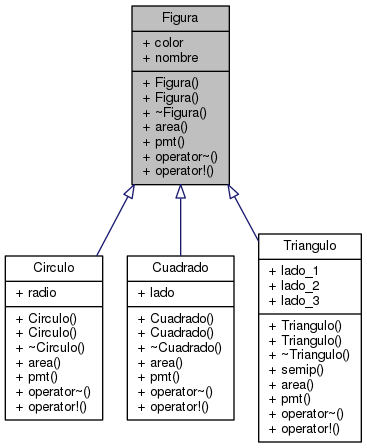
\includegraphics[scale=0.9]{class_figura__inherit__graph.png}
	\label{fig:UML}
\end{figure}
\vspace{2 em}

\section{Conclusiones}
\begin{enumerate}
	\item Una clase derivada hereda los atributos y métodos públicos de la clase base.
	\item Los métodos virtuales de la clase base son los que se pueden reimplementar en las clases derivadas.
	\item La sobrecarga de operadores facilita la implementación de métodos.	
\end{enumerate}
\end{document}
